\documentclass{beamer}
\usepackage[utf8]{inputenc}
\usepackage{graphicx}
\usetheme{Madrid}
\usecolortheme{default}
\usepackage[export]{adjustbox}
\usepackage{amsmath,amssymb}
\usepackage{hyperref}
\usepackage{listings}
\DeclareRobustCommand{\bbone}{\text{\usefont{U}{bbold}{m}{n}1}}

\setbeamertemplate{navigation symbols}{} 
\date{MAY 3,2023}
\DeclareMathOperator{\EX}{\mathbb{E}}% expected value
%------------------------------------------------------------
%This block of code defines the information to appear in the
%Title page
\title[R-Tree] %optional
{R-Tree}


\author[] % (optional)
{Dhyey Italiya - 2021A7PS1463P\\Saurabh Bhandari - 2021A7PS2412P\\ Saksham Verma - 2021A7PS2414P\\Lakshit Sethi - 2021A7PS2434P\\Abir Abhyankar - 2021A7PS0523P}

\institute[BITS Pilani] % (optional)
{
  Birla Institute of Technology and Science,Pilani\\
  Dr.Jagat Sesh Challa
}

%End of title page configuration block
%------------------------------------------------------------


%------------------------------------------------------------
%The next block of commands puts the table of contents at the 
%beginning of each section and highlights the current section

\AtBeginSection[]
{
  \begin{frame}
    \frametitle{Table of Contents}
    \tableofcontents[currentsection]
  \end{frame}
}
%------------------------------------------------------------


\begin{document}

%The next statement creates the title page.
\frame{\titlepage}


%---------------------------------------------------------
%This block of code is for the table of contents after
%the title page
\begin{frame}
\frametitle{Table of Contents}
\tableofcontents
\end{frame}
%---------------------------------------------------------

\section{Introduction}
\begin{frame}
\frametitle{R-Tree Structure}
\begin{itemize}
    \item M - Maximum number of Entries in each Node.
    \item m - Minimum number of Entries in each Node.
    \item MBR - Minimum Bounding Rectangle.It contains two pairs of integers which defines the bounds along X-axis and Y-axis
    \item Node - It contains an array of Entries whose size is bounded by the values of M and m.It also stores a pointer to its Parent Node and parent Entry.
    \item Entry - It contains an MBR and a pointer to its child node.\bigskip
    
    Each node has a boolean isLeaf which checks whether it is a leaf node or not.
\end{itemize}
\end{frame}

\begin{frame}
\frametitle{R-Tree Structure}
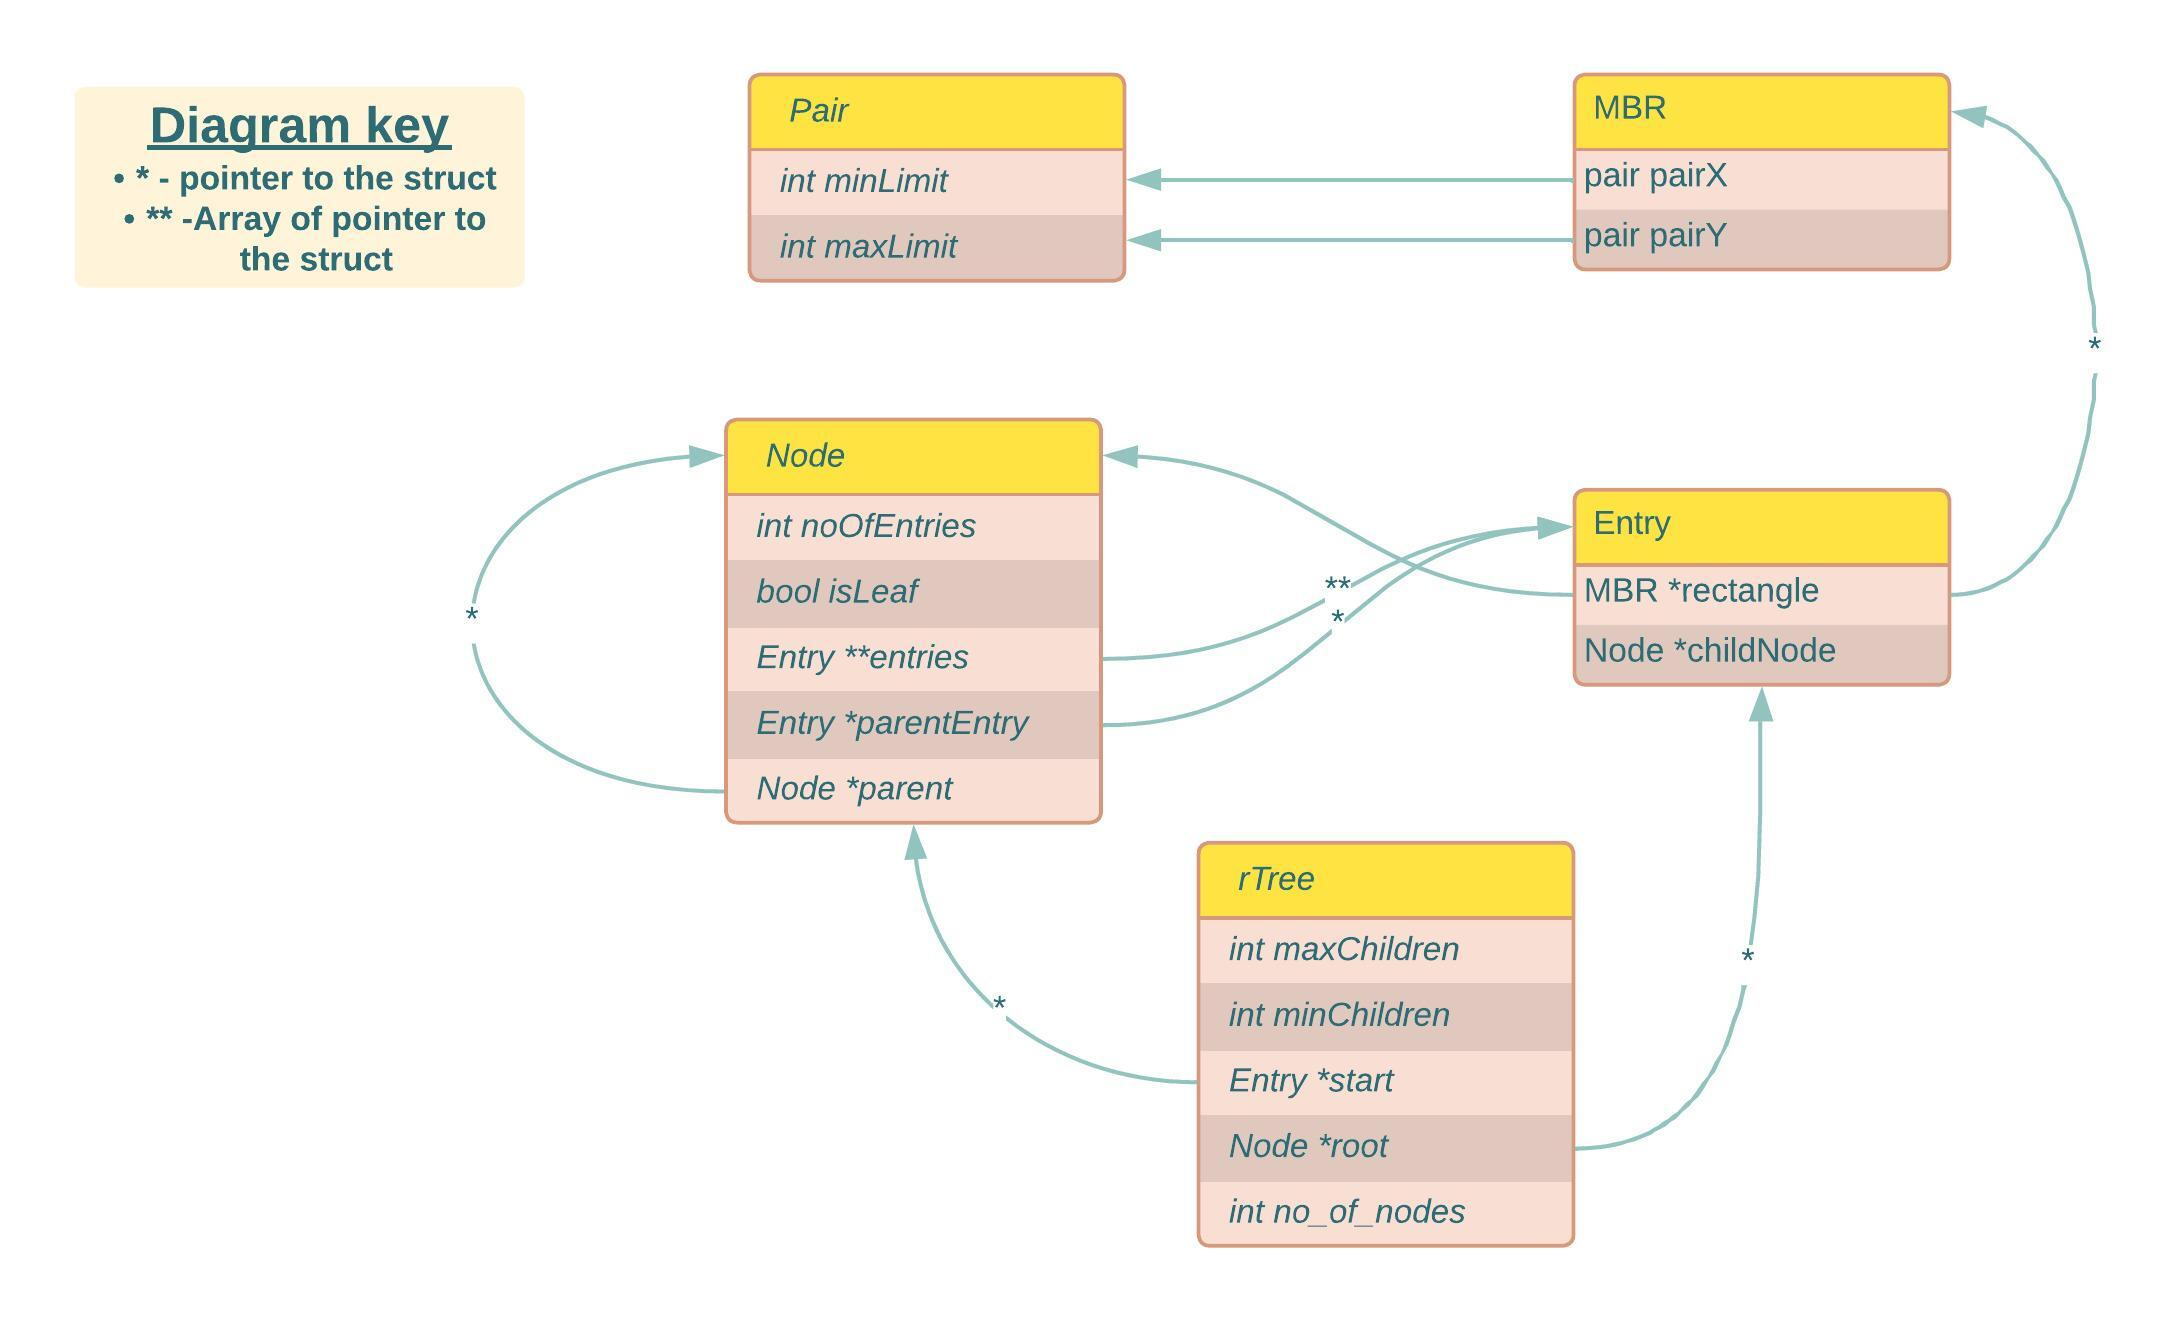
\includegraphics[scale=0.7,center]{Structs_relations.jpeg}
\end{frame}

\begin{frame}{R-Tree Structure}
    \begin{block}{MBR}
    Minimum Bounding Rectangle.It contains two pairs of integers which defines the bounds along X-axis and Y-axis
         \includegraphics[scale=0.25,center]{MBR_struct.png}
    \end{block}
    \begin{block}{Node}
    It contains an array of Entries whose size is bounded by the values of M and m.It also stores a pointer to its Parent Node and parent Entry.
         \includegraphics[scale=0.25,center]{Node_struct.png}
    \end{block}
\end{frame}

\end{frame}
\begin{frame}{R-Tree Structure}
    \begin{block}{Entry}
    It contains an MBR and a pointer to its child node.
         \includegraphics[scale=0.25,center]{Entry_struct.png}
    \end{block}
    \begin{block}{R-tree}
         \includegraphics[scale=0.25,center]{rTree_struct.png}
    \end{block}
\end{frame}
%------------------------------------------------------------------------
\section{Functions}
\begin{frame}{Functions}
\begin{itemize}
    \item Traversal - We have implemented Preorder Traversal which first prints the node and then its children from left to right.
    \bigskip
    \item Search - It searches for leaf MBRs that overlaps with a given MBR.
    \bigskip
    \item Insert - Insert a given MBR into the tree.
    \bigskip
\end{itemize}
\end{frame}
%-------------------------
\begin{frame}{Traversal}
    \begin{itemize}
        \item The function preOrderTraversal is used to traverse an R-Tree in Pre-Order.
    
        \bigskip
        \item The function preOrderTraversal uses an auxiliary function named preOrderTraversal\_Utility.
        
        \bigskip 
        \item preOrderTraversal\_Utility in turn uses the printNode function.
        
        \bigskip
        \item printNode traverses through the node and prints each entry stored in it with the help of the printEntry function.
    \end{itemize}
\end{frame}
%-------------------------
\begin{frame}{Traversal_{preOrderTraversal}}
    This function uses an auxiliary function named preOrderTraversal\_Utility.
    
    The preOrderTraversal function takes the R-Tree and starts traversing it in Pre-Order.
    
    It passes the root of the R-Tree to the preOrderTraversal\_Utility function for traversal.
    
    \begin{block}{PreOrder Traversal}
        \includegraphics[scale=0.25,center]{preOrderTraversal_func.png}
    \end{block}
\end{frame}
%-------------------------
\begin{frame}{Traversal_{preOrderTraversal\_Utility}}
    This function uses an auxiliary function named printNode.
    
    The preOrderTraversal\_Utility function takes a Node and prints it using the printNode function.
    
    It passes the current node to the printNode function.
    
    It traverses through the children of the current node from left to right and recursively calls itself on the children for Pre-Order traversal.
    
    \begin{block}{PreOrderTraversal\_Utility}
        \includegraphics[scale=0.25,center]{preOrderTraversalUtility_func.png}
    \end{block}
\end{frame}
%-------------------------
\begin{frame}{Traversal_{printNode}}
    This function uses an auxiliary function named printEntry.
    
    The printNode function takes a node and prints all the entries in the node.
    
    The function also prints the Node Number of the Child Nodes of the entries contained in it.
    
    It passes the entries of the node one-by-one to the printEntry function for printing the MBR of the entry.
    
    \begin{block}{PrintNode}
        \includegraphics[scale=0.25,center]{printNode_func.png}
    \end{block}
\end{frame}
%-------------------------
\begin{frame}{Traversal_{printEntry}}
    The printEntry function takes an entry and prints the Top-Right and Bottom-Left points of the MBR stored in the entry.
    
    The function does not print anything if the MBR of the entry is NULL.
    
    \begin{block}{PrintEntry}
        \includegraphics[scale=0.25,center]{printEntry_func.png}
    \end{block}
\end{frame}
%-------------------------
\begin{frame}{Search}
    The function search uses an auxilliary function search utility.
    
    The search utility function takes the current node and a MBR as input.
    \begin{block}{search utility}
       \begin{itemize}
           \item If the Current Node is NULL,it returns the function.
           \item If the Current Node is a leaf,the function searches all the entries in the node and prints the entries which overlap.
           \item If the Current Node is not a leaf,It searches all the enteries and call the search utility function for the child node of all the enteries which overlap.
       \end{itemize}
    \end{block}
\end{frame}
%--------------------------
\begin{frame}{Search}
       This is a wrapper function which the user uses in order to search an R-Tree.

       The search function takes the R-Tree and the values of the MBR as input.
       \begin{block}{search}
       \begin{itemize}
           \item The function creates a MBR using the values provided.
           \item The function then calls the search utility function giving the tree's root as the current node and the MBR created as input.
       \end{itemize}

       
    \end{block}
\end{frame}
%-----------------------------
\begin{frame}{Insertion_{chooseLeaf}}
    \begin{block}{chooseLeaf}
       \includegraphics[scale=0.35,center]{chooseLeaf1_func.png}
    \end{block}
\end{frame}
%-----------------------------
\begin{frame}{Insertion_{chooseLeaf}}
    \begin{block}{chooseLeaf contd.}
       \includegraphics[scale=0.35,center]{chooseLeaf2_func.png}
    \end{block}
\end{frame}
%-----------------------------
\begin{frame}{Insertion_{pickSeeds}}
    \begin{block}{pickSeeds}
       \includegraphics[scale=0.40,center]{pickSeeds1_func.png}
    \end{block}
\end{frame}
%-----------------------------
\begin{frame}{Insertion_{pickSeeds}}
    \begin{block}{pickSeeds contd.}
       \includegraphics[scale=0.35,center]{pickSeeds2_func.png}
    \end{block}
\end{frame}
%-----------------------------
\begin{frame}{Insertion_{pickNext}}
int pickNext(Node *currNode, Entry *group1, Entry *group2, bool *res)
    \begin{block}{pickNext}
       \includegraphics[scale=0.25,center]{pickNext_funcfor.png}
    \end{block}
\end{frame}
%-----------------------------
\begin{frame}{Insertion_{QuadraticSplit}}
void quadraticSplit(Node *currNode, rTree *tree)
    \begin{block}{QuadraticSplit}
       \includegraphics[scale=0.30,center]{QuadSplit1_func.png}
    \end{block}
\end{frame}
%-----------------------------
\begin{frame}{Insertion_{QuadraticSplit}}
Iterating through all the entries of given node with a while loop as:\\
while (currNode --$>$ noOfEntries $>$ 0)\\
Picking the next entry to be added to a group, and the group to which it should be added.
    \begin{block}{QuadraticSplit contd.}
       \includegraphics[scale=0.30,center]{QuadSplit2_func.png}
    \end{block}
\end{frame}
%-----------------------------
\begin{frame}{Insertion_{QuadraticSplit}}
Handling the case where one of the groups has maxChildren entries,we add all the remaining entries to the other group.
    \begin{block}{QuadraticSplit contd.}
       \includegraphics[scale=0.35,center]{QuadSplit3_func.png}
    \end{block}
\end{frame}
%-----------------------------
\begin{frame}{Insertion_{QuadraticSplit}}
If the current node is the root node, create a new root node and add the groups as its children.
    \begin{block}{QuadraticSplit contd.}
       \includegraphics[scale=0.35,center]{QuadSplit4_func.png}
    \end{block}
\end{frame}
%-----------------------------
\begin{frame}{Insertion_{QuadraticSplit}}
Else add the groups as entries to the parent node and remove the current node.
    \begin{block}{QuadraticSplit contd.}
       \includegraphics[scale=0.35,center]{QuadSplit5_func.png}
    \end{block}
\end{frame}
%-----------------------------
\begin{frame}{Insertion_{adjustTree}}
Adjusts the tree after insertion
    \begin{block}{adjustTree}
       \includegraphics[scale=0.40,center]{adjTree1_func.png}
    \end{block}
\end{frame}
%-----------------------------
\begin{frame}{Insertion_{adjustTree}}
Adjust the MBR of the parent node and check if it needs to be split and update the MBR of the parent node.\\
\bigskip
If the parent node needs to be split, split it and adjust the tree again.
    \begin{block}{adjustTree contd.}
       \includegraphics[scale=0.30,center]{adjTree2_func.png}
    \end{block}
\end{frame}
%-----------------------------
\begin{frame}{Insertion}
    \begin{block}{insert}
       \includegraphics[scale=0.35,center]{insert_func.png}
    \end{block}
\end{frame}
%-----------------------------
\end{document}
